\section{寄存器描述}
\regover{
{\hyperref[spi-spi-config]{spi\_config}}&Master and slave configure
\\
\hline
{\hyperref[spi-spi-int-sts]{spi\_int\_sts}}&Interrupt configure and status
\\
\hline
{\hyperref[spi-spi-bus-busy]{spi\_bus\_busy}}&Bus busy status
\\
\hline
{\hyperref[spi-spi-prd-0]{spi\_prd\_0}}&Period configure 0
\\
\hline
{\hyperref[spi-spi-prd-1]{spi\_prd\_1}}&Period configure 1
\\
\hline
{\hyperref[spi-spi-rxd-ignr]{spi\_rxd\_ignr}}&RX ignore function
\\
\hline
{\hyperref[spi-spi-sto-value]{spi\_sto\_value}}&Timer-out value setting
\\
\hline
{\hyperref[spi-spi-fifo-config-0]{spi\_fifo\_config\_0}}&FIFO status and DMA mode
\\
\hline
{\hyperref[spi-spi-fifo-config-1]{spi\_fifo\_config\_1}}&FIFO threshold and available count
\\
\hline
{\hyperref[spi-spi-fifo-wdata]{spi\_fifo\_wdata}}&TX FIFO
\\
\hline
{\hyperref[spi-spi-fifo-rdata]{spi\_fifo\_rdata}}&RX FIFO
\\
\hline
{\hyperref[spi-backup-io-en]{backup\_io\_en}}&IO backup
\\
\hline
}

\subsection{spi\_config}
\label{spi-spi-config}
地址:0x40019000
 \begin{figure}[H]
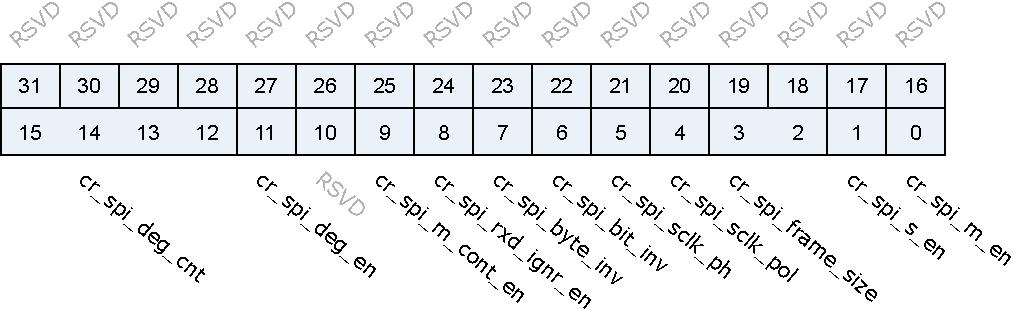
\includegraphics{spi_spi_config.pdf}
\end{figure}

\regdes{31:16&RSVD& & & \\\hline
15:12&cr\_spi\_deg\_cnt&r/w&4'd0&De-glitch function cycle count\\\hline
11&cr\_spi\_deg\_en&r/w&1'b0&Enable signal of all input de-glitch function\\\hline
10&cr\_spi\_s\_3pin\_mode&r/w&1'b0&SPI slave 3-pin mode \par 1'b0: 4-pin mode (SS\_n is enabled) \par 1'b1: 3-pin mode (SS\_n is disabled / don't care)
\\\hline
9&cr\_spi\_m\_cont\_en&r/w&1'b0&Enable signal of master continuous transfer mode \par 1'b0: Disabled, SS\_n will de-assert between each data frame \par 1'b1: Enabled, SS\_n will stay asserted between each consecutive data frame if the next data is valid in the FIFO
\\\hline
8&cr\_spi\_rxd\_ignr\_en&r/w&1'b0&Enable signal of RX data ignore function\\\hline
7&cr\_spi\_byte\_inv&r/w&1'b0&Byte-inverse signal for each FIFO entry data \par 0: Byte[0] is sent out first \par 1: Byte[3] is sent out first(32-bit frame size) / byte[2] is send out first(24-bit frame size) / byte[1] is send out first(16-bit frame size)
\\\hline
6&cr\_spi\_bit\_inv&r/w&1'b0&Bit-inverse signal for each data byte \par 0: Each byte is sent out MSB-first \par 1: Each byte is sent out LSB-first
\\\hline
5&cr\_spi\_sclk\_ph&r/w&1'b0&SCLK clock phase inverse signal \par 0: Data is sampled on the second edge of SCLK  \par 1: Data is sampled on the first edge of SCLK
\\\hline
4&cr\_spi\_sclk\_pol&r/w&1'b0&SCLK polarity \par 0: SCLK output LOW at IDLE state \par 1: SCLK output HIGH at IDLE state
\\\hline
3:2&cr\_spi\_frame\_size&r/w&2'd0&SPI frame size (also the valid width for each FIFO entry) \par 2'd0: 8-bit, FIFO space is 1*32 = 32 byte \par 2'd1: 16-bit, FIFO space is 2*16 = 32 byte \par 2'd2: 24-bit, FIFO space is 3*8 = 24 byte \par 2'd3: 32-bit, FIFO space is 4*8 = 32 byte
\\\hline
1&cr\_spi\_s\_en&r/w&1'b0&Enable signal of SPI Slave function, Master and Slave should not be both enabled at the same time \par (This bit becomes don't-care if cr\_spi\_m\_en is enabled)
\\\hline
0&cr\_spi\_m\_en&r/w&1'b0&Enable signal of SPI Master function \par Asserting this bit will trigger the transaction, and should be de-asserted after finish
\\\hline

}
\subsection{spi\_int\_sts}
\label{spi-spi-int-sts}
地址:0x40019004
 \begin{figure}[H]
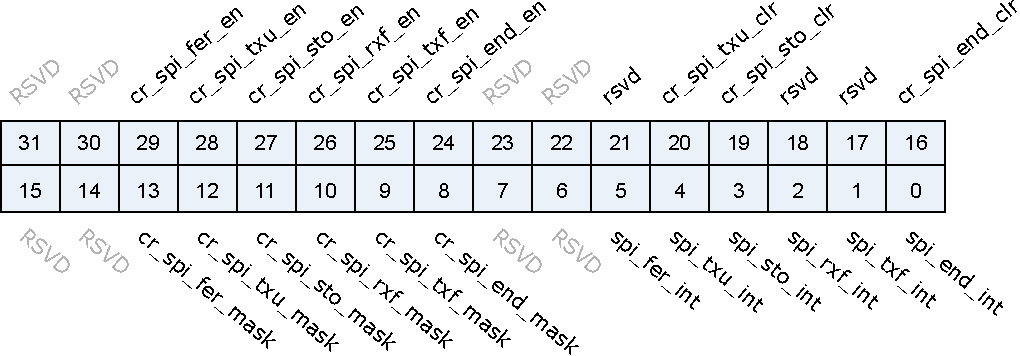
\includegraphics{spi_spi_int_sts.pdf}
\end{figure}

\regdes{31:30&RSVD& & & \\\hline
29&cr\_spi\_fer\_en&r/w&1'b1&Interrupt enable of spi\_fer\_int\\\hline
28&cr\_spi\_txu\_en&r/w&1'b1&Interrupt enable of spi\_txu\_int\\\hline
27&cr\_spi\_sto\_en&r/w&1'b1&Interrupt enable of spi\_sto\_int\\\hline
26&cr\_spi\_rxf\_en&r/w&1'b1&Interrupt enable of spi\_rxv\_int\\\hline
25&cr\_spi\_txf\_en&r/w&1'b1&Interrupt enable of spi\_txe\_int\\\hline
24&cr\_spi\_end\_en&r/w&1'b1&Interrupt enable of spi\_end\_int\\\hline
23:22&RSVD& & & \\\hline
21&rsvd&rsvd&1'b0&\\\hline
20&cr\_spi\_txu\_clr&w1c&1'b0&Interrupt clear of spi\_txu\_int\\\hline
19&cr\_spi\_sto\_clr&w1c&1'b0&Interrupt clear of spi\_sto\_int\\\hline
18&rsvd&rsvd&1'b0&\\\hline
17&rsvd&rsvd&1'b0&\\\hline
16&cr\_spi\_end\_clr&w1c&1'b0&Interrupt clear of spi\_end\_int\\\hline
15:14&RSVD& & & \\\hline
13&cr\_spi\_fer\_mask&r/w&1'b1&Interrupt mask of spi\_fer\_int\\\hline
12&cr\_spi\_txu\_mask&r/w&1'b1&Interrupt mask of spi\_txu\_int\\\hline
11&cr\_spi\_sto\_mask&r/w&1'b1&Interrupt mask of spi\_sto\_int\\\hline
10&cr\_spi\_rxf\_mask&r/w&1'b1&Interrupt mask of spi\_rxv\_int\\\hline
9&cr\_spi\_txf\_mask&r/w&1'b1&Interrupt mask of spi\_txe\_int\\\hline
8&cr\_spi\_end\_mask&r/w&1'b1&Interrupt mask of spi\_end\_int\\\hline
7:6&RSVD& & & \\\hline
5&spi\_fer\_int&r&1'b0&SPI TX/RX FIFO error interrupt, auto-cleared when FIFO overflow/underflow error flag is cleared\\\hline
4&spi\_txu\_int&r&1'b0&SPI slave mode TX underrun error flag, triggered when TXD is not ready during transfer in slave mode\\\hline
3&spi\_sto\_int&r&1'b0&SPI slave mode transfer time-out interrupt, triggered when SPI bus is idle for a given value\\\hline
2&spi\_rxf\_int&r&1'b0&SPI RX FIFO ready (rx\_fifo\_cnt > rx\_fifo\_th) interrupt, auto-cleared when data is popped\\\hline
1&spi\_txf\_int&r&1'b1&SPI TX FIFO ready (tx\_fifo\_cnt > tx\_fifo\_th) interrupt, auto-cleared when data is pushed\\\hline
0&spi\_end\_int&r&1'b0&SPI transfer end interrupt, shared by both master and slave mode \par Master mode: Triggered when the final frame is transferred \par Slave mode: Triggered when CS\_n is de-asserted
\\\hline

}
\subsection{spi\_bus\_busy}
\label{spi-spi-bus-busy}
地址:0x40019008
 \begin{figure}[H]
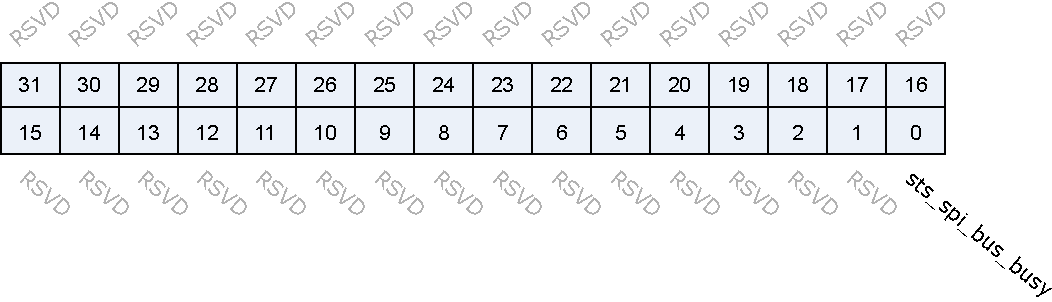
\includegraphics{spi_spi_bus_busy.pdf}
\end{figure}

\regdes{31:1&RSVD& & & \\\hline
0&sts\_spi\_bus\_busy&r&1'b0&Indicator of SPI bus busy \par 0: Idle \par 1: Busy
\\\hline

}
\subsection{spi\_prd\_0}
\label{spi-spi-prd-0}
地址:0x40019010
 \begin{figure}[H]
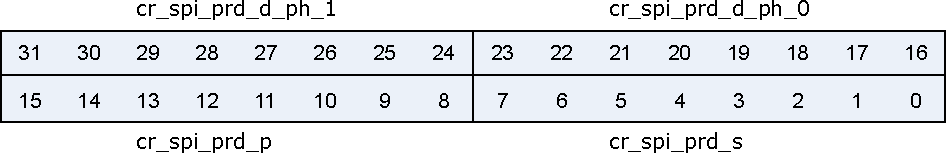
\includegraphics{spi_spi_prd_0.pdf}
\end{figure}

\regdes{31:24&cr\_spi\_prd\_d\_ph\_1&r/w&8'd15&Length of DATA phase 1 (unit: SPI source clock period)\\\hline
23:16&cr\_spi\_prd\_d\_ph\_0&r/w&8'd15&Length of DATA phase 0 (unit: SPI source clock period)\\\hline
15:8&cr\_spi\_prd\_p&r/w&8'd15&Length of STOP condition (unit: SPI source clock period)\\\hline
7:0&cr\_spi\_prd\_s&r/w&8'd15&Length of START condition (unit: SPI source clock period)\\\hline

}
\subsection{spi\_prd\_1}
\label{spi-spi-prd-1}
地址:0x40019014
 \begin{figure}[H]
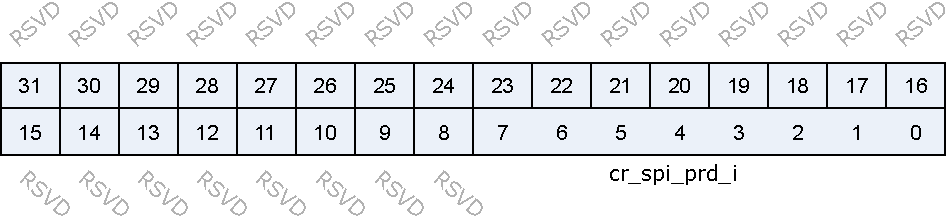
\includegraphics{spi_spi_prd_1.pdf}
\end{figure}

\regdes{31:8&RSVD& & & \\\hline
7:0&cr\_spi\_prd\_i&r/w&8'd15&Length of INTERVAL between frame (unit: SPI source clock period)\\\hline

}
\subsection{spi\_rxd\_ignr}
\label{spi-spi-rxd-ignr}
地址:0x40019018
 \begin{figure}[H]
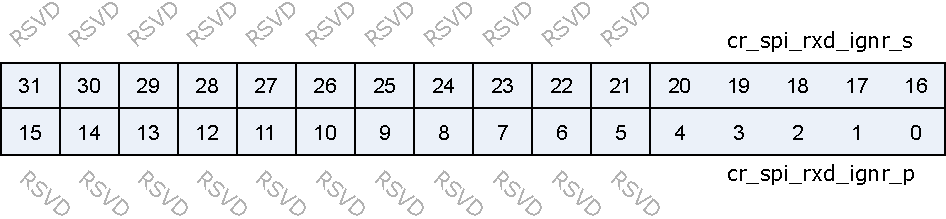
\includegraphics{spi_spi_rxd_ignr.pdf}
\end{figure}

\regdes{31:21&RSVD& & & \\\hline
20:16&cr\_spi\_rxd\_ignr\_s&r/w&5'd0&Starting point of RX data ignore function (unit: bit)\\\hline
15:5&RSVD& & & \\\hline
4:0&cr\_spi\_rxd\_ignr\_p&r/w&5'd0&Stopping point of RX data ignore function (unit: bit)\\\hline

}
\subsection{spi\_sto\_value}
\label{spi-spi-sto-value}
地址:0x4001901c
 \begin{figure}[H]
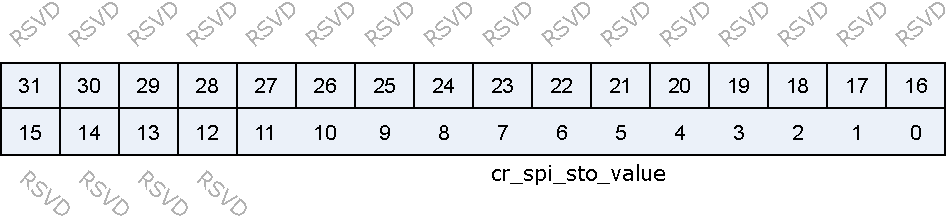
\includegraphics{spi_spi_sto_value.pdf}
\end{figure}

\regdes{31:12&RSVD& & & \\\hline
11:0&cr\_spi\_sto\_value&r/w&12'hFFF&Time-out value for spi\_sto\_int triggering\\\hline

}
\subsection{spi\_fifo\_config\_0}
\label{spi-spi-fifo-config-0}
地址:0x40019080
 \begin{figure}[H]
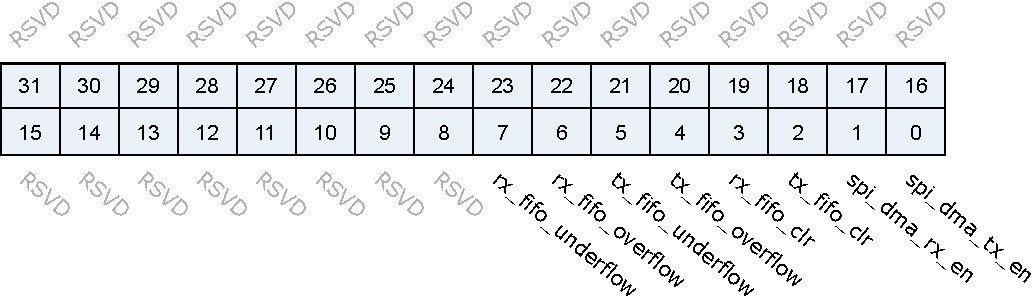
\includegraphics{spi_spi_fifo_config_0.pdf}
\end{figure}

\regdes{31:8&RSVD& & & \\\hline
7&rx\_fifo\_underflow&r&1'b0&Underflow flag of RX FIFO, can be cleared by rx\_fifo\_clr\\\hline
6&rx\_fifo\_overflow&r&1'b0&Overflow flag of RX FIFO, can be cleared by rx\_fifo\_clr\\\hline
5&tx\_fifo\_underflow&r&1'b0&Underflow flag of TX FIFO, can be cleared by tx\_fifo\_clr\\\hline
4&tx\_fifo\_overflow&r&1'b0&Overflow flag of TX FIFO, can be cleared by tx\_fifo\_clr\\\hline
3&rx\_fifo\_clr&w1c&1'b0&Clear signal of RX FIFO, RX FIFO will be empty when write 1 to this bit\\\hline
2&tx\_fifo\_clr&w1c&1'b0&Clear signal of TX FIFO, TX FIFO will be empty when write 1 to this bit\\\hline
1&spi\_dma\_rx\_en&r/w&1'b0&Enable signal of dma\_rx\_req/ack interface\\\hline
0&spi\_dma\_tx\_en&r/w&1'b0&Enable signal of dma\_tx\_req/ack interface\\\hline

}
\subsection{spi\_fifo\_config\_1}
\label{spi-spi-fifo-config-1}
地址:0x40019084
 \begin{figure}[H]
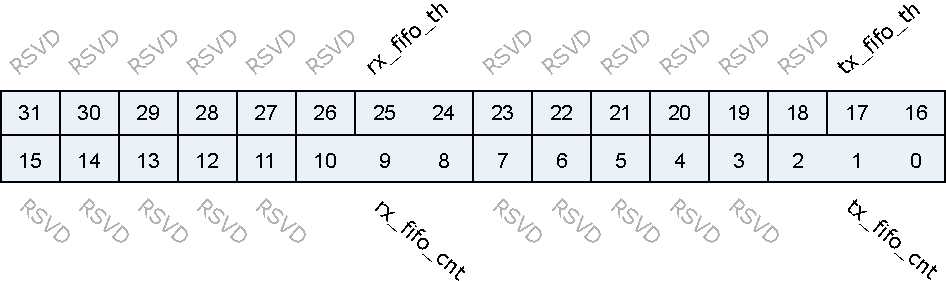
\includegraphics{spi_spi_fifo_config_1.pdf}
\end{figure}

\regdes{31:29&RSVD& & & \\\hline
28:24&rx\_fifo\_th&r/w&5'd0&RX FIFO threshold, dma\_rx\_req will not be asserted if rx\_fifo\_cnt is less than this value\\\hline
23:21&RSVD& & & \\\hline
20:16&tx\_fifo\_th&r/w&5'd0&TX FIFO threshold, dma\_tx\_req will not be asserted if tx\_fifo\_cnt is less than this value\\\hline
15:14&RSVD& & & \\\hline
13:8&rx\_fifo\_cnt&r&6'd0&RX FIFO available count, means byte count of data received in RX FIFO (unit: byte)\\\hline
7:6&RSVD& & & \\\hline
5:0&tx\_fifo\_cnt&r&6'd32&TX FIFO available count, means empty space remained in TX FIFO (unit: byte)\\\hline

}
\subsection{spi\_fifo\_wdata}
\label{spi-spi-fifo-wdata}
地址:0x40019088
 \begin{figure}[H]
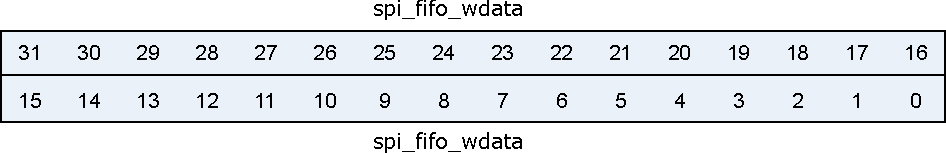
\includegraphics{spi_spi_fifo_wdata.pdf}
\end{figure}

\regdes{31:0&spi\_fifo\_wdata&w&x&TX FIFO write data port \par Note: Partial valid if cr\_spi\_frame\_size is set to different value: \par 2'd0 (8-bit frame): Only [7:0] are valid and [31:8] are don't-care \par 2'd1 (16-bit frame): Only [15:0] are valid and [31:16] are don't-care \par 2'd2 (24-bit frame): Only [23:0] are valid and [31:24] are don't-care \par 2'd3 (32-bit frame): Entire [31:0] are valid
\\\hline

}
\subsection{spi\_fifo\_rdata}
\label{spi-spi-fifo-rdata}
地址:0x4001908c
 \begin{figure}[H]
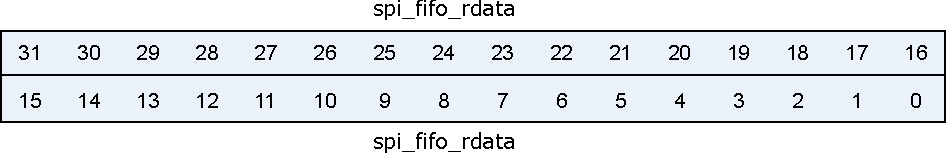
\includegraphics{spi_spi_fifo_rdata.pdf}
\end{figure}

\regdes{31:0&spi\_fifo\_rdata&r&32'h0&RX FIFO read data port \par Note: Partial valid if cr\_spi\_frame\_size is set to different value: \par 2'd0 (8-bit frame): Only [7:0] are valid and [31:8] are all 0s \par 2'd1 (16-bit frame): Only [15:0] are valid and [31:16] are all 0s \par 2'd2 (24-bit frame): Only [23:0] are valid and [31:24] are all 0s \par 2'd3 (32-bit frame): Entire [31:0] is valid
\\\hline

}
\subsection{backup\_io\_en}
\label{spi-backup-io-en}
地址:0x400190fc
 \begin{figure}[H]
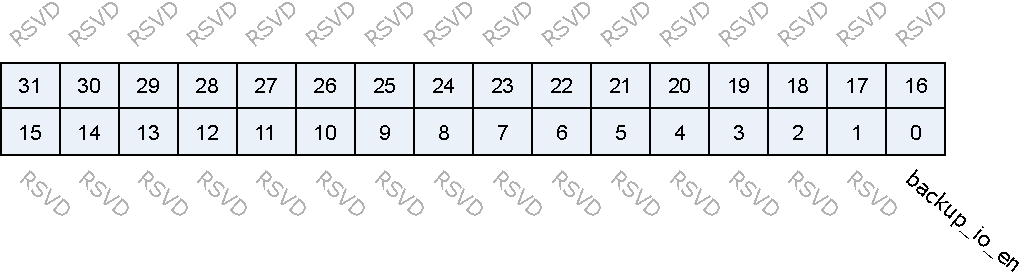
\includegraphics{spi_backup_io_en.pdf}
\end{figure}

\regdes{31:1&RSVD& & & \\\hline
0&backup\_io\_en&r/w&1'b0&Enable IO backup function\\\hline

}
